\subsection{Phân tích phương sai một nhân tố (Single-factor ANOVA)}
Mục tiêu: Đánh giá xem biến nhân tố X có ảnh hưởng đến biến phụ thuộc Y hay không?
%mùa ảnh hưởng tới phí giao hàng
    Chúng em quyết định sẽ kiểm định xem, việc các mùa (season) sẽ ảnh hưởng như thế nào đến phí giao hàng (delivery\_charges) bằng
phương pháp phân tích phương sai ANOVA một nhân tố. Dưới đây là phân tích phương sai ANOVA một nhân tố cho mẫu thống kê ( hàm phân tích đã được tích hợp sẵn trong R) :

\begin{figure}[!htbp]
    \centering
    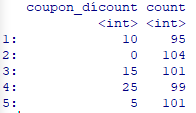
\includegraphics[width=0.7\linewidth]{graphics/5.3.1.png}
    \caption{Phân tích phương sai ANOVA xét sự ảnh hưởng của mùa (season) đến phí giao hàng(delivery\_charges)}
\end{figure}

    Xem hình trên ta thấy kết quả, giá trị p-value (tức Pr(>F)) là rất rất nhỏ hơn ngưỡng ý nghĩa phổ biến (0.05). Do đó, cho thấy sự
khác biệt rất có ý nghĩa thống kê, có đủ bằng chứng thống kê rất mạnh để kết luận rằng, các mùa (season) có ảnh hưởng rất mạnh đến phí giao hàng (delivery\_charges).
%yêu cầu giao hàng nhanh ảnh hưởng tới phí giao hàng

    Tiếp theo chúng em quyết định sẽ tiếp tục kiểm định thêm một yếu tố nữa là việc khách hàng yêu cầu giao hàng nhanh (is\_expedited\_delivery) sẽ ảnh hưởng như thế nào đến phí giao hàng (delivery\_charges) bằng phương pháp phân tích phương sai ANOVA một nhân tố. Dưới đây là phân tích phương sai ANOVA một nhân tố cho mẫu thống kê ( hàm phân tích đã được tích hợp sẵn trong R) :
\begin{figure}[!htbp]
    \centering
    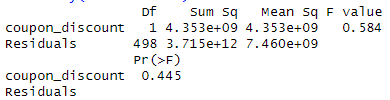
\includegraphics[width=0.7\linewidth]{graphics/5.3.2.png}
    \caption{Phân tích phương sai ANOVA xét sự ảnh hưởng của việc khách hàng yêu cầu giao hàng nhanh (is\_expedited\_delivery) đến phí giao hàng(delivery\_charges)}
\end{figure}

    Xem hình trên ta thấy kết quả, giá trị p-value (tức Pr(>F)) là rất rất nhỏ hơn ngưỡng ý nghĩa phổ biến (0.05). Do đó, cho thấy sự
khác biệt rất có ý nghĩa thống kê, có đủ bằng chứng thống kê rất mạnh để kết luận rằng, việc khách hàng yêu cầu giao hàng nhanh (is\_expedited\_delivery) có ảnh hưởng rất mạnh đến phí giao hàng (delivery\_charges).
